\documentclass{standalone}
\usepackage{tikz}
\usepackage{ctex,siunitx}
\setCJKmainfont{Noto Serif CJK SC}
\usepackage{tkz-euclide}
\usepackage{amsmath}
\usetikzlibrary{patterns, calc}
\usetikzlibrary {decorations.pathmorphing, decorations.pathreplacing, decorations.shapes,}

\begin{document}
\small
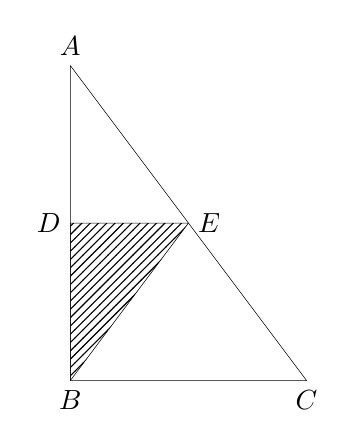
\begin{tikzpicture}[>=stealth,scale=1.0]
  \tkzSetUpPoint[fill=black]
  % \useasboundingbox(-1,-0.75)rectangle(3.7,1.4);
  \tkzDefPoints{0/0/B, 3/0/C, 0/4/A}
  \tkzDefMidPoint(A,B)\tkzGetPoint{D}
  \tkzDefMidPoint(A,C)\tkzGetPoint{E}
  \tkzDrawPolygon(A,B,C)
  \tkzDrawPolygon[pattern=north east lines](B,D,E)
  \tkzLabelPoints[right](E)
  \tkzLabelPoints[left](D)
  \tkzLabelPoints[below](B,C)
  \tkzLabelPoints[above](A)
\end{tikzpicture}
\end{document}